\documentclass[compress,10pt,aspectratio=169]{beamer}
\usetheme[customnumbering]{onera}

\usepackage{amsmath,amsfonts,graphicx}
\usepackage{pifont}
\usepackage{etoolbox}
\usepackage{multicol}
\usepackage{anyfontsize}
\usepackage{multirow}
\usepackage{hyperref}
\usepackage{amsmath}
\usepackage{colortbl}
\usepackage{tcolorbox}
\usepackage{fontspec}
%\setlength{\columnseprule}{1pt}
%\def\columnseprulecolor{\color{blue}}
\usepackage{minted} % syntax coloring. 
\setminted{encoding=utf-8, autogobble, fontsize=\scriptsize, frame=single}
\usemintedstyle{xcode}

\usepackage{stackengine}
%\AtBeginEnvironment{minted}{\fontsize{8}{8}\selectfont}

%\usepackage{dsfont}
\usepackage{ifdraft}
\ifdraft{
  \usepackage{fancyvrb}
  \DefineVerbatimEnvironment{cppcode}{Verbatim}{}
}{
\newminted{cpp}{}
}
\usepackage{hyperref}
\usetikzlibrary{shadows, arrows, decorations.pathmorphing, fadings, shapes.arrows, positioning, calc, shapes, fit, matrix,math}

\definecolor{lightblue}{RGB}{0,200,255} 
\definecolor{paper}{RGB}{255,247,197}
\definecolor{ocre}{RGB}{243,102,25} % Define the orange color used for highlighting throughout the book
\definecolor{BurntOrange}{RGB}{238,154,0}
\definecolor{darkorange}{RGB}{119, 77, 0}
\definecolor{OliveGreen}{RGB}{188,238,104}
\definecolor{DarkGreen}{RGB}{0,128,0}
\definecolor{BrickRed}{RGB}{238,44,44}
\definecolor{Tan}{RGB}{210,180,140}
\definecolor{Aquamarine}{RGB}{127,255,212}
\definecolor{NavyBlue}{RGB}{0,64,128}
\definecolor{DarkYellow}{RGB}{192,192,0}
\definecolor{Yellow}{RGB}{255,255,0}

\title[Initiation C++\hspace{2em}]{Programmation orientée objet}
\subtitle{POO}
\author[X. JUVIGNY]{Xavier JUVIGNY, AKOU, DAAA, ONERA\\ \href{mailto:xavier.juvigny@onera.fr}{\texttt{xavier.juvigny@onera.fr}} }
\date[04/11/2023]{Initiation au C++ \\- 4 Novembre 2023 -}
\institute{\inst{1}ONERA,\inst{2}DAAA}

\AtBeginSection[]{
  \begin{frame}{Overview}
  \begin{multicols}{2}
  \small \tableofcontents[currentsection, hideallsubsections]
  \end{multicols}
  \end{frame} 
}

\begin{document}

\begin{frame}
 \titlepage
\end{frame}

\begin{frame}
\frametitle{Plan du cours}
\tableofcontents
\end{frame}

\section{Introduction à l'orienté objet}

\begin{frame}[fragile]{Orienté Objets}
    \scriptsize
    \begin{block}{Programmation orienté objets}
    \begin{itemize}
    \item Un style de programmation, une façon de programmer
    \begin{itemize}
    \scriptsize
    \item Avec un langage traditionnel;
    \item Avec un langage orienté objets
    \end{itemize}
    \end{itemize}
    \alert{Programmer avec un langage OO ne fait pas de l'orienté objets}
    \end{block}


    \begin{block}{Définition de l'objet}
    \begin{itemize}
    \item Un objet contient à la fois des données et des fonctions faisant des traitements sur ces données.
    \item Autres concepts similaires aux autres méthodes de programmation.
    \item Un jargon à connaître :
    \end{itemize}
    \begin{tabular}{|c|c|c|}\hline
    Type & Variable & Valeurs \\ \hline
    \textcolor{orange}{Classe} & \textcolor{orange}{Variable} & \textcolor{orange}{Valeurs/Objets} \\ \hline
    \mintinline{C++}{class Vecteur;} & \mintinline{C++}{int u; double x;} & \mintinline{C++}{[1.,3.,5.], "Coucou",  23, Vecteur(1.,3.,5.,7.)} \\ \hline
    \end{tabular}
    \end{block}
    \end{frame}
   
    \begin{frame}[fragile]{Service vs réalisation}
        \scriptsize
        \begin{block}{\small Objectif}
        \begin{itemize}
        \item Une valeur qui représente un nuage de points : Un ensemble de couples X et Y, réels
        \item De nombreuses réalisations sont possibles.
      \begin{exampleblock}{\small Exemple d'interface}
        \begin{itemize}
          \scriptsize
          \item Un vecteur de X, un autre de Y, même taille
        \item Un vecteur de couples (X,Y)
        \item Avec un dictionnaire : Chaque point avec une clef $(i,j)$ et le couple $(x,y)$ en valeur ou un vecteur de X et un vecteur de Y avec une clef par zone, par exemple les $X>0$, les $X<0$ et les $X==0$
        \end{itemize}
      \end{exampleblock}
        \item Pour chaque mise en œuvre\ldots
        \begin{itemize}
          \scriptsize
          \item Une fonction qui retourne les X, une les Y
        \item Donne le nombre de points
        \item Une qui donne tous les points, au dessus/au dessous d'un X ou d'un Y, avec une valeur exacte de X
        \end{itemize}
      \end{itemize}
      \end{block}
        \end{frame}

\begin{frame}[fragile]{La donnée pilote l'algorithme}
  \scriptsize
\begin{multicols}{2}
\begin{minipage}{0.5\textwidth}
\begin{block}{\small Exemple avec choix de réalisation n°1}
\begin{minted}{C++}
auto coords=std::make_pair(std::vector<double>{100},
                           std::vector<double>{100});
using coordinates=decltype(coords);
auto& y = coords.second;
auto yLowerThan(const coordinates& crds,double val){
  coordinates c; 
  std::vector<int> r;
  for ( int i = 0; i < crds.first.size(); ++i) {
    if (crds.second[i] < val ) {
      c.first.push_back(crds.first[i]); 
      c.second.push_back(crds.second[i]);
      r.push_back(i);
    }
  }
  return std::make_tuple(c,r);
}
\end{minted}
\end{block}
\end{minipage}
\columnbreak
\begin{minipage}{0.5\textwidth}
\begin{exampleblock}{\small Exemple avec choix de réalisation n°2}
\begin{minted}{C++}
using coordinates=std::vector<std::pair<double,
                                        double>>;
coordinates coords(100);
std::vector<double> y(100); 
for (int iy=0; const auto& c : coords ) 
    y[++iy] = c.second;
auto yLowerThan(const coordinates& crds,double val){
  coordinates c; 
  std::vector<int> r; 
  for ( int i = 0; i < crds.size(); ++i) {
    if (crds[i].second < val ) {
      c.push_back(crds[i]); r.push_back(i);
    }  
  }
  return std::make_tuple(c,r); 
}
\end{minted}
\end{exampleblock}
\end{minipage}
\end{multicols}
\end{frame}

\begin{frame}[fragile]{Concrétisation de l'interface}
    \scriptsize
    \begin{block}{\small Homogénéité de l'interface}
    \begin{itemize}
    \item Divers objets possèdent la même interface :
    \begin{itemize}
    \scriptsize
    \item Des objets de même type : réels, entiers, etc.
    \item Les listes, les tableaux, les dictionnaires, etc :
    \end{itemize}
    \end{itemize}
    \end{block}
  \begin{minted}{C++}
    std::vector<double>  u{ {3.4, 5.8, 1.2} };
    std::list<double>    l{ {3.4, 5.8, 1.2} };
    std::array<3,double> a{ {3.4, 5.8, 1.2} };
    
    for ( auto& val : u) val *= 0.5;
    for ( auto& val : l) val *= 0.5;
    for ( auto& val : a) val *= 0.5;
    
    u.push_back(2.);
    l.push_back(2.);
  \end{minted}
    \end{frame}
  
    \begin{frame}[fragile]{Mise en {\oe}uvre d'une interface}
        \scriptsize
        \begin{exampleblock}{\small Mise au point de l'interface}
        Méthode de développement TDD ( Test Driven Development ) :
        \begin{itemize}
        \item L'interface se conçoit en écrivant les tests de "haut niveau" en premier lieu;
        \item On regarde avec le client si l'interface proposé dans les tests correspond à son attente.
        \end{itemize}
        \end{exampleblock}
      
        \begin{block}{\small Mise au point d'une identité vecteur géométrique}
        \begin{minted}{C++}
        #include "vecteur.hpp"
        
        Geometry::Vecteur u{ { 1., 0., 0. } };
        Geometry::Vecteur v;
        v.x = u.z; v.y = -u.x; v.z = u.y
        
        std::cout << u << " + " << v << " = " << u+v << std::endl;
        double nrmSq_u = u.normalize(); double nrmSq_v = v.normalize();
        Geometry::Vecteur w = u - (u|v)*v;
        \end{minted}
        \alert{En premier lieu, bien définir son interface}
        \end{block}
        
        \begin{block}{\small Conception d'une classe}
        \begin{itemize}
        \item \textcolor{violet}{Concevoir une classe n'est pas un fin en soi}
        \item C'est \textbf{un} moyen de réaliser une interface ( mais on peut utiliser d'autres techniques si elles sont plus adaptées ).
        \end{itemize}
        \end{block}
        
\end{frame}
      
\begin{frame}{Conception d'une interface}
    \scriptsize
    \begin{minipage}{0.59\textwidth}
    \begin{block}{\small Interface-1}
    \begin{itemize}
    \item Que la partie utilisable de l'objet :
    \begin{itemize}
    \scriptsize
    \item Accès aux données pertinentes de l'objet;
    \item Des constantes;
    \item Des fonctions ( méthodes ) pour manipuler l'objet;
    \item Gestion du comportement;
    \end{itemize}
    \item \textcolor{orange}{Un exemple} : Le téléphone
    \end{itemize}
    \end{block}
    \end{minipage}
    \begin{minipage}{0.39\textwidth}
    \begin{center}
    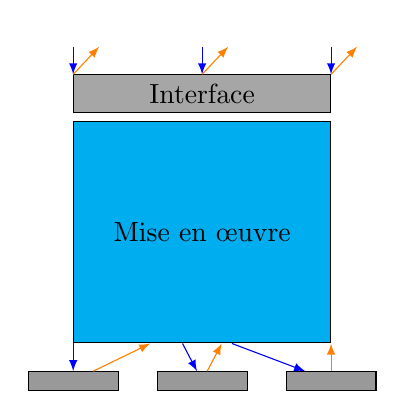
\begin{tikzpicture}
    \node[draw,fill=gray!70, text width=20ex, text centered] (I) {Interface};
    \node[draw,fill=cyan, text width=20ex,minimum height = 8em, below=1mm of I.south, text centered] (M) {Mise en {\oe}uvre};
    \node[draw,fill=gray!80, text width=6ex, below=1em of M.south west] (Im1) {};
    \node[draw,fill=gray!80, text width=6ex, below=1em of M.south] (Im2) {};
    \node[draw,fill=gray!80, text width=6ex, below=1em of M.south east] (Im3) {};
    \node[above=1em of I.north west] (E1) {};
    \node[above=1em of I.north] (E2) {};
    \node[above=1em of I.north east] (E3) {};
    \node[right=2mm of E1] (E11) {};
    \node[right=2mm of E2] (E21) {};
    \node[right=2mm of E3] (E31) {};
    \draw[blue,-latex] (E1) -- (I.north west);
    \draw[blue,-latex] (E2) -- (I.north);
    \draw[blue,-latex] (E3) -- (I.north east);
    \draw[orange,-latex] (I.north west) -- (E11) ;
    \draw[orange,-latex] (I.north) -- (E21);
    \draw[orange,-latex] (I.north east) -- (E31);
    
    \draw[blue,-latex] (M.south west) -- (Im1);
    \draw[orange,-latex] (Im1) -- (M.245);
    
    \draw[blue,-latex] (M.260) -- (Im2);
    \draw[orange,-latex] (Im2) -- (M.280);
    
    \draw[blue,-latex] (M.285) -- (Im3);
    \draw[orange,-latex] (Im3) -- (M.south east);
    \end{tikzpicture}
    \end{center}
    \end{minipage}
\end{frame} 

\begin{frame}[fragile]{Conception d'une interface (2)}
    \scriptsize
    \begin{minipage}{0.59\textwidth}
    \begin{block}{\small Fonctions}
    \begin{itemize}
    \item \mintinline{C++}{status:int initialize()}
    \item \mintinline{C++}{value:float currentData(variable:string)}
    \item \mintinline{C++}{terminate()}
    \end{itemize}
    \alert{Plusieurs variables pour currentData ?}
    \end{block}
    \vspace*{-5mm}
    \begin{block}{\small Constantes}
    \begin{itemize}
    \item \mintinline{C++}{variables = ["Temperature", "Pressure"]}
    \end{itemize}
    \end{block}
  
    \vspace*{-5mm}
    \begin{block}{\small Comportement}
    \begin{itemize}
    \item créer l'objet
    \item initialize (commence l'échantillonage)
    \item currentData (si status est True)
    \item terminate (arrêt échantillonage)
    \item détruire l'objet
    \end{itemize}
    \alert{\underline{Quid gestion des erreurs ?} Bad initialization, Timeout, \ldots}
    \end{block}
    \end{minipage}
    \begin{minipage}{0.39\textwidth}
    \begin{center}
    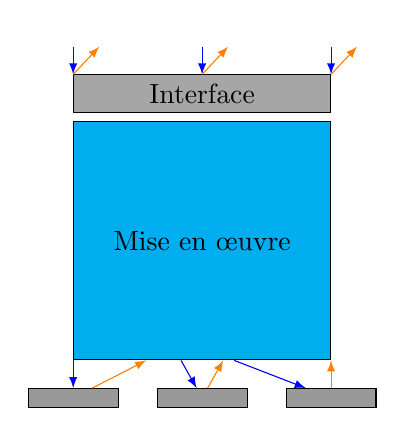
\begin{tikzpicture}
    \node[draw,fill=gray!70, text width=20ex, text centered] (I) {Interface};
    \node[draw,fill=cyan, text width=20ex, minimum height = 20ex, below=1mm of I.south, text centered] (M) {Mise en {\oe}uvre};
    \node[draw,fill=gray!80, text width=6ex, below=1em of M.south west] (Im1) {};
    \node[draw,fill=gray!80, text width=6ex, below=1em of M.south] (Im2) {};
    \node[draw,fill=gray!80, text width=6ex, below=1em of M.south east] (Im3) {};
    \node[above=1em of I.north west] (E1) {};
    \node[above=1em of I.north] (E2) {};
    \node[above=1em of I.north east] (E3) {};
    \node[right=2mm of E1] (E11) {};
    \node[right=2mm of E2] (E21) {};
    \node[right=2mm of E3] (E31) {};
    \draw[blue,-latex] (E1) -- (I.north west);
    \draw[blue,-latex] (E2) -- (I.north);
    \draw[blue,-latex] (E3) -- (I.north east);
    \draw[orange,-latex] (I.north west) -- (E11) ;
    \draw[orange,-latex] (I.north) -- (E21);
    \draw[orange,-latex] (I.north east) -- (E31);
    
    \draw[blue,-latex] (M.south west) -- (Im1);
    \draw[orange,-latex] (Im1) -- (M.245);
    
    \draw[blue,-latex] (M.260) -- (Im2);
    \draw[orange,-latex] (Im2) -- (M.280);
    
    \draw[blue,-latex] (M.285) -- (Im3);
    \draw[orange,-latex] (Im3) -- (M.south east);
    \end{tikzpicture}
    \end{center}
    \end{minipage}
    \end{frame}
  
    \begin{frame}[fragile]{Conception d'une interface (3)}
        \scriptsize
        \begin{block}{\small Comportement}
        \begin{minipage}{0.59\textwidth}
        Généralement décrit par un automate.
        \end{minipage}
        \begin{minipage}{0.39\textwidth}
        \begin{center}
        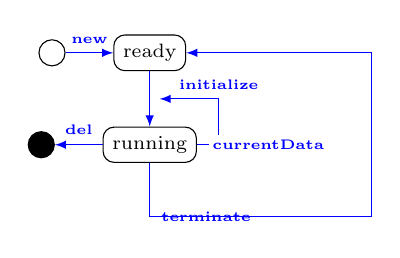
\begin{tikzpicture}
        \node[draw,circle] (start) {};
        \node[draw,rectangle,rounded corners=4pt, right=4ex of start.east] (ready){\scriptsize ready};
        \node[draw,rectangle,rounded corners=4pt, below=2em of ready.south] (running){\scriptsize running};
        \node[right=1ex of running.east] (ar1){};
        \node[draw,circle,fill=black, left=4ex of running.west] (stop){};
        \draw[->,>=latex,blue] (start) -- node[midway, above]{\tiny\bf new}(ready);
        \draw[->,>=latex,blue] (ready) -- node[midway](inte){} (running);
        \draw[->,>=latex,blue] (running) -- node[midway,above]{\tiny\bf del} (stop);
        \draw[->,>=latex,blue] (running) -- node[below,right]{\tiny\bf currentData} (ar1) |- node[midway,above]{\tiny\bf initialize} (inte);
        \draw[->,>=latex,blue] (running) -- +(0,-6ex) -- node[below,left]{\tiny\bf terminate} +(8em,-6ex) |- (ready.east);
        \end{tikzpicture}
        \end{center}
        \end{minipage}
        \end{block}
        \begin{multicols}{2}
        \begin{block}{\small Interface N+1}
        Interface utilisant les services offerts par l'interface.\\
        \textbf{Exemple} : Interface visualisation données envoyées par capteurs.
        \end{block}
        \columnbreak
        \begin{block}{\small Interface N-1}
        Interface utilisée ( non unique ) par l'interface actuelle
        \begin{itemize}
        \item Se traduit en C++ par un \mintinline{C++}{#include}
        \item Ou par un appel système
        \end{itemize}
        \end{block}
      \end{multicols}
        \end{frame}

\begin{frame}{Principes de l'OO}
  \scriptsize
  \begin{multicols}{2}
  \begin{minipage}{0.49\textwidth}
  \begin{block}{\small L'interface}
  Les services offerts à l'extérieur du module/bibliothèque
  \end{block}
  \begin{block}{\small L'encapsulation}
  Isoler/Cacher les choix de mises en {\oe}uvres
  \end{block}
\end{minipage}
  \columnbreak
  \begin{minipage}{0.49\textwidth}
    \begin{block}{\small La factorisation}
  Factoriser les services communs au sein de types "abstraits"
  \begin{itemize}
  \item Polymorphisme
  \item \textsl{Héritage}
  \end{itemize}
  \end{block}
  
  \begin{alertblock}{\small Mises en {\oe}uvre}
  Réalisable dans tous les langages de programmation.\\
  Les langages OO fournissent des facilités.
  \end{alertblock}
\end{minipage}
\end{multicols}
  \end{frame}

\begin{frame}{Encapsulation}
  \scriptsize
  \begin{block}{\scriptsize Une unité}
  Un paquet comprenant tout ce qu'on peut trouver pour installer une bibliothèque/module qui contient :
  \begin{itemize}
  \item des données;
  \item des traitements sur les données;
  \item mais aussi :
  \begin{itemize}
  \scriptsize
  \item des constantes;
  \item traitement des erreurs;
  \item des tests
  \item de la documentation
  \item la production
  \end{itemize}
  \end{itemize}
  \end{block}
  
  \begin{block}{\small Mise en {\oe}uvre}
  Le choix de ce qui est dans l'objet ou pas est arbitraire. Il dépend de l'application. Il n'est pas possible de définir un objet idéal pour toutes les applications. C'est donc différent d'une modélisation mathématique.
  \end{block}
  \end{frame}
  
  \begin{frame}[fragile]{OO -- Principes -- Isolation}
  \scriptsize

  \begin{multicols}{2}
  \begin{block}{\small Une interface}
  Les services, les fonctions, les constantes,\ldots
  \end{block}
  \columnbreak  
  \begin{block}{\small Une réalisation}
  \begin{itemize}
  \item La structure interne des valeurs manipulées;
  \item La mise en œuvre effective des services.
  \end{itemize}
  \end{block}
\end{multicols}
  
  \begin{block}{\small La règle d'or}
  \alert{\bf Ne pas exposer la réalisation}
  
  \begin{minipage}{0.49\textwidth}
  \begin{minted}{C++}
  double retrieveCurrentMax( const Capteur& a ) {
      return a.max;
  }
  \end{minted}
  
  \begin{minted}{C++}
  double retrieveCurrentMax( const Capteur& a ) {
      a.update(); return a.max;
  }
  \end{minted}
  \end{minipage}
  \begin{minipage}{0.49\textwidth}
  \begin{minted}{C++}
  double retrieveCurrentMax( const Capteur& a ) {
      return std::min(a.max, CONST_VAL_MAX);
  }
  \end{minted}
  \begin{minted}{C++}
  double retrieveCurrentMax( const Capteur& a ) {
      return CONST_VAL_MAX;
  }
  \end{minted}
  \end{minipage}
  \end{block}
  \end{frame}

  \begin{frame}[fragile]{OO -- Principes -- Factorisation }
    \scriptsize
  
    \begin{multicols}{2}
    \begin{block}{\small Si deux objets sont similaires}
    \begin{itemize}
    \item Et ont une partie de leurs interfaces commune;
    \item Possible de factoriser cette partie de l'interface;
    \item Permet d'éviter de la duplication de code 
    \item $\Rightarrow$ facilite la maintenance du code.
    \end{itemize}
    \end{block}
    \columnbreak  
    \begin{exampleblock}{\small \underline{Exemple}: Les matrices}
    \begin{itemize}
    \item Matrice inversible est une matrice carrée (factorisable);
    \item Matrice carrée est une matrice (multipliable par un vecteur);
    \item Matrice est un tableau à deux dimensions \\(accès c{\oe}fs par indices ligne/colonne)
    \end{itemize}
    \end{exampleblock}
  \end{multicols}
    
    \begin{alertblock}{\small Règle à suivre}
    Si \textbf{B} est un sous-ensemble de \textbf{A}, alors \textbf{b} est au moins un \textbf{a}.
    
    \textsl{\textcolor{blue}{Mais... Si je peux rajouter une ligne à une matrice, que doit faire une matrice carrée ?}}
    \end{alertblock}
    \end{frame}
    
    \begin{frame}{Principes -- Factorisation -- 2}
    \scriptsize
    \begin{block}{\small Deux grandes règles de base pour les classes}
    \begin{itemize}
    \item La factorisation se conçoit sur les objets, puis se formalise sur les classes;
    \item La factorisation est arbitraire : elle dépend de l'application visée.
    \end{itemize}
    \end{block}
    
    \begin{alertblock}{\small Erreurs traditionnelles de la conception des classes}
    \begin{itemize}
    \item Il ne s'agit pas de modéliser le monde !
    \item Il s'agit seulement de réaliser du code pour une application.
    \end{itemize}
    \end{alertblock}
    \end{frame}
    
    \begin{frame}{OO - Principes -- Factorisation -- 3}
    \scriptsize
    \begin{block}{\small Règle de base de l'OO}
    \textbf{L'encapsulation} et son corollaire immédiat et essentiel : \textbf{l'interface}
    \end{block}
    \vspace*{-2mm}
    \begin{block}{\small La factorisation}
    \textsl{Matrice inversible, matrice carrée, matrice,\ldots}\\
    \begin{itemize}
    \item La factorisation des interfaces donne la hiérarchie des classes;
    \item Factoriser seulement les valeurs utilisables;
    \item Généralisation
    \item À ne pas confondre avec la \textbf{composition}.
    \end{itemize}
    \end{block}
    \vspace*{-2mm}
    
    \begin{block}{\small La dérivation}
    \textsl{Matrice inversible, matrice symétrique inversible}
    \begin{itemize}
    \item Ne dériver que les valeurs utilisables;
    \item Spécialisation
    \end{itemize}
    \end{block}
    \end{frame}

\begin{frame}[fragile]{Hiérarchie des classes}
  \scriptsize
  \begin{block}{\small Factorisation/Dérivation des types}
  \begin{itemize}
  \item Forme une arborescence 
  \begin{itemize}
  \scriptsize
  \item Une matrice carrée est une matrice;
  \item Une matrice symétrique est une matrice carrée;
  \item Une matrice symétrique définie positive est une matrice symétrique;
  \item Une matrice inversible est une matrice carrée; 
  \end{itemize}
  \end{itemize}
  \end{block}
  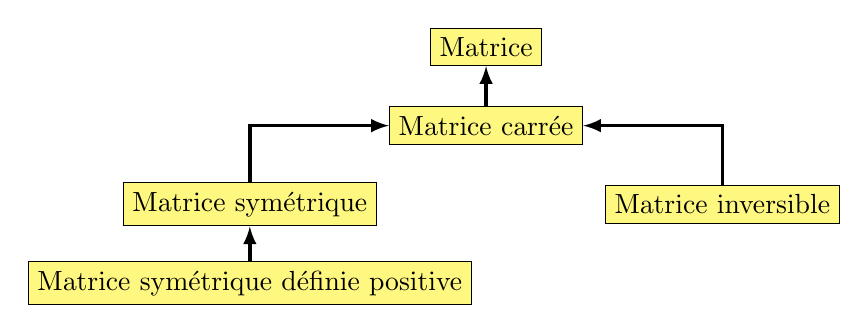
\begin{tikzpicture}
  \tikzstyle{class} = [rectangle,fill=yellow!50,draw]
  \tikzstyle{estun} = [->, very thick, >=latex]
  \node[class] at (0,5) (M) {Matrice};
  \node[class] at (0,4) (C) {Matrice carrée};
  \node[class] at (-3,3) (S) {Matrice symétrique};
  \node[class] at (+3,3) (I) {Matrice inversible};
  \node[class] at (-3,2) (SDP) {Matrice symétrique définie positive};
  \draw[estun] (C) -- (M);
  \draw[estun] (S) |- (C);
  \draw[estun] (I) |- (C);
  \draw[estun] (SDP) -- (S);
  \end{tikzpicture}
  \end{frame}

\section{POO en C++}

\begin{frame}[fragile]{Syntaxe de déclaration de la classe}
    \scriptsize
    \begin{block}{\small Déclaration}
  \begin{minted}{C++}
  class Vecteur //<--- Déclaration d'un nouveau type Vecteur
  {
  public: // Partie accessible par une fonction externe à la classe
    Vecteur() = default;//Constructeur par défaut
    void setAsPoint();// Méthode publique de la classe
    double x,y,z;// Attributs publics de la classe
  private: // Partie privée accessible uniquement aux méthodes de la classe.
    bool is_point() const; // Méthode privée de la classe
    double w; // Attributs privés de la classe
  };
  Vecteur u;// <-- Nouvelle variable de type Vecteur faisant appel au constructeur par défaut
  u.x = 3.0;//Accès aux attributs publiques de la classe
  u.y = 2.0; u.z = 1.0;
  u.setAsPoint();// Appel d'une méthode setAsPoint appliquée au vecteur u
  \end{minted}
  \end{block}
  \vspace*{-2mm}
  On a ici définit un constructeur par défaut qui ne fait que réserver la mémoire pour les trois attributs $x,y$ et $z$
  \end{frame}

\begin{frame}[fragile]{Les constructeurs}
  \scriptsize
  \vspace*{-3mm}
  \begin{block}{\small Les constructeurs}
    \vspace*{-3mm}
    \begin{multicols}{2}
      \begin{itemize}
  \item Décrit façon d'initialiser variable du type qu'on définit;
  \item Il doit être nommé du même nom que le type;
  \item Plusieurs constructeurs possibles avec liste d'arguments différents;
  \end{itemize}
\end{multicols}
\end{block}
  \begin{minted}{C++}
  class Vecteur {
  public:
    Vecteur();// Constructeur par défaut
    // Initialisation du vecteur à partir d'une liste de valeurs
    Vecteur( const std::initializer_list<double>& init_vals );
    Vecteur( double cx, double cy, double cz  );//Initialisation à partir de 3 entiers
    Vecteur( double cx );//Initialisation à partir de 1 réel
    Vecteur( const Vecteur& u ); // Constructeur de copie
    Vecteur( Vecteur&& u ); // Constructeur de déplacement
    ... //D'autres constructeurs si on le souhaite...
  };  
  Vecteur u;                 // Appel au constructeur par défaut
  Vecteur v{ {1., 3., -5.} };// Appel construction avec liste d'initialisation
  Vecteur w( 3., 4., 2.);  // Appel constructeur avec trois réels
  Vecteur z(1.); // Appel contructeur avec un réel
  Vecteur y(z);// Appel le constructeur de copie
  Vecteur w(std::move(y)); // Appel constructeur de déplacement
  \end{minted}
  \end{frame}

  \begin{frame}[fragile]{Les constructeurs}
    \scriptsize
    \begin{block}{\small Règles du C++ sur les constructeurs}
    \begin{itemize}
      \item Si aucun constructeur déclaré, C++ définit constructeur par défaut sans 
            paramètres, appelant constructeurs par défaut de chaque attribut de la classe;
      \item Si non déclaré, C++ définit constructeur de copie et constructeur de déplacement 
            appelant les constructeurs de copie/déplacement de chacun des attributs;
      \item Si un des attributs non copiable ( respectivement non déplaçable ), alors 
            constructeur de copie ( resp. de déplacement ) automatiquement supprimé;
      \item Possible d'appeler un constructeur dans liste d'initialisation ( voir plus 
            loin ) d'un autre constructeur de la même classe (C++11).
    \end{itemize}
    \alert{Toujours déclarer les trois constructeurs : celui 
           par défaut ( sans paramètre ), celui de copie et celui de déplacement, quitte à les 
           déclarer par défaut ou supprimés ( voir transparent suivant ).}
    \end{block}
    \end{frame}
    
    \begin{frame}[fragile]{Les constructeurs par défauts}
    \scriptsize
    \begin{block}{\small Constructeurs par défaut}
      \begin{itemize}
        \item Valable uniquement pour constructeur sans paramêtre, copie et déplacement;
        \item Rajouter \mintinline{C++}{= default} à la fin de la déclaration;
        \item Constructeur par défaut effectue comportement par défaut :
        \begin{itemize}
        \scriptsize
        \item Constructeur sans paramêtre : Appelle constructeur sans paramêtre pour chaque attribut.
              Pour les valeurs de type "basique", valeurs non initialisées.
        \item Constructeur de copie : Appelle constructeur de copie pour chaque attribut;
        \item Constructeur de déplacement : Appelle constructeur de déplacement pour chaque attribut.
        \end{itemize}
      \end{itemize}
    \end{block}
    
    \begin{minted}{C++}
    class Vecteur {
    public:
      Vecteur()                   = default; // Le tableau m_valeurs sera construit vide
      Vecteur( const Vecteur& u ) = default; // Clone le tableau de u dans Vecteur en construction
            ...
    private:
      std::vector<double> m_valeurs;
    };
    \end{minted}
    \end{frame}  
    
    \begin{frame}[fragile]{Les constructeurs par défauts supprimés}
    \scriptsize
    
    \begin{block}{\small Interdire la création implicite d'un constructeur par défaut}
    \begin{itemize}
    \item Le C++ peut définir implicitement des constructeurs par défaut 
          (voir~\ref{reglesConstructeur});
    \item Et si on ne veut pas que ces constructeurs soient définis ?
    \item On peut explicitement interdire un constructeur d'être implicitement défini
          en le déclarant et en rajoutant à la fin de la déclaration \mintinline{c++}{= delete};
    \end{itemize}
    \end{block}
      
    \begin{minted}{C++}
    class Vecteur {
    public:
      Vecteur() = default;// Constructeur sans paramétre par défaut
      Vecteur( const Vecteur& u ) = default;//Construction de copie par défaut
      Vecteur( Vecteur&& u ) = delete;//Interdiction de déplacer
          ...
    private:
      std::vector<double> m_valeurs;
    };
    \end{minted}
    \end{frame}
      
    \begin{frame}[fragile]{Mise en {\oe}uvre d'un constructeur}
    \scriptsize
    \begin{block}{\small Constructeur en ligne}
    On peut définir un constructeur dans la déclaration de la classe $\Rightarrow$ déclaré en ligne (inline)
    \begin{minted}{C++}
    // vecteur.hpp
    class Vecteur {
      ...
      //                           initialisation des attributs   ---\ 
      //                                                             ↓
      Vecteur( const std::initializer_list<double>& vals ) : m_valeurs{vals} {}   
      Vecteur( double x, double y, double z );//<--- seulement déclarée !
      ...
      private:
      std::array<double,3> m_valeurs;
    };
    \end{minted}
    La définition du constructeur doit y être brêve !
    \end{block}
    \end{frame}
    
    \begin{frame}[fragile]{Mise en {\oe}uvre d'un constructeur (suite)}
    \scriptsize
    \begin{block}{\small Mise en {\oe}uvre d'un constructeur}
    Pour un constructeur uniquement déclaré au sein de la déclaration de la classe, on peut :
    \begin{itemize}
    \item le définir en ligne dans le fichier de déclaraction (.hpp) 
    \begin{minted}{c++}
    // vecteur.hpp après déclaration de la classe
    inline Vecteur::Vecteur( double x, double y, double z ) : m_valeurs{} {
      m_valeurs[0] = x; m_valeurs[1] = y; m_valeurs[2] = z;
    }
    \end{minted}
    \item le définir dans le fichier de mise en {\oe}uvre (.cpp)
    \begin{minted}{c++}
    // vecteur.cpp
    # include "vecteur.hpp"
    // Pour toutes méthodes/attributs définis en dehors de la classe :
    // Nom de la classe :: Nom de la méthode/attribut
    Vecteur::Vecteur( double x, double y, double z ) : m_valeurs{} {
      m_valeurs[0] = x; m_valeurs[1] = y; m_valeurs[2] = z;
    }
    \end{minted}
    \end{itemize}
    \end{block}
    \end{frame}
      
    \begin{frame}[fragile]{Constructeur de copie/de déplacement}
    \scriptsize
    \vspace*{-3mm}
    \begin{block}{\small Constructeur de copie}
    \begin{itemize}
      \item Pour créer un nouvel objet en copiant les valeurs d'un objet existant;
      \item Utilisé implicitement lors passage paramêtre par valeur ou retour
            par valeur d'une valeur non locale à une fonction
    \end{itemize}
    
    \begin{minted}{c++}
    class Vecteur {
      ...
      Vecteur( const Vecteur& u ) : m_valeurs(u.m_valeurs) {}
      ...
    };
    \end{minted}
    \end{block}
    \vspace*{-3mm}
    \begin{block}{\small Constructeur de déplacement}
    \begin{itemize}
      \item Créer nouvel objet en y déplaçant valeurs d'un objet existant,
            ancien objet ne possèdera plus ces données;
      \item Utilisé lors du retour par valeur d'une fonction d'une variable locale à cette fonction.
    \end{itemize}
    \begin{minted}{c++}
    class Vecteur {
      ...
      Vecteur( Vecteur&& u ) : m_valeurs(std::move(u.m_valeurs))
      {}
    };
    \end{minted}
    \end{block}
    \end{frame}

\begin{frame}[fragile]{Destructeur}
  \scriptsize
  \begin{block}{\small Déclaration du destructeur}
  \begin{itemize}
    \item Permet de définir la façon dont un objet du type de la classe va se détruire;
    \item Peut être définit par défaut : appel le destructeur correspondant à chacune des valeurs de l'objet;
    \item déclaré avec le même nom que la classe précédé d'un \verb@~@.
    \item \textcolor{orange}{Un seul destructeur par classe}. Ne possède pas de paramètres;
    \item Appelé avant la sortie du bloc de visibilité de l'objet.
  \end{itemize}
  \end{block}
  \begin{minted}{c++}
class Vecteur { 
  ...
  ~Vecteur() = default;
};
\end{minted}
\end{frame}
      
\begin{frame}[fragile]{Gestion des exceptions pour les constructeurs {\color{red}\bf\Large (+)}}
  \scriptsize
  \begin{block}{\small Gestion des exceptions lors de la construction}
    Utiliser le bloc \mintinline{c++}{try... catch} autour de l'initialisation de l'objet :
  \begin{multicols}{2}
  \begin{minipage}{0.49\textwidth}
  \begin{minted}{C++}
  class Matrix { 
  public: 
    ...
    Matrix( int nrows, int ncols );
    ...
  private: 
    std::vector<double> m_valeurs; 
  };
  Matrix::Matrix( int nrows, int ncols ) try :
    m_valeurs(nrows*ncols)//<--- Liste initialisation
  { ... // Corps du constructeur.
  }
  catch(std::bad_alloc& err) {
    ...
    throw std::bad_alloc(errMsg);
  }
  \end{minted}
  \end{minipage}
  \begin{minipage}{0.49\textwidth}
    \begin{itemize}
    \item Impossible de rattraper une exception au sein d'un constructeur;
    \item Rattraper une exception pour un constructeur ne peut servir qu'à le reinterpréter et le renvoyer.
    \item L'objet n'existe pas lors du traitement de l'exception.
  \end{itemize}
  \end{minipage}
  \end{multicols}
  \end{block}
  \end{frame}
    
  \begin{frame}[fragile]{Gestion des erreurs dans un constructeur{\color{red}\bf\Large (+)}}
  \scriptsize
  \begin{block}{Exceptions}
  \begin{itemize}
    \item Seul moyen propre de signaler les erreurs dans un constructeur;
    \item Si une exception est levée, l'objet ne sera \textbf{jamais créé};
    \item L'objet est créé uniquement au moment de quitter le constructeur;
    \item Exception dans sous-objet ( attribut/héritage ) : objet non construit;
    \item Pour une sous-partie optionelle, utiliser l'idiome de mise en {\oe}uvre \textbf{Pimpl}.
  \end{itemize}
  \end{block}
  \begin{minipage}{0.6\textwidth}
  \begin{minted}{c++}
  // CapteurPression.hpp
  class CapteurPression {
       ...
  private:
    PressureSensor m_pressure;
    ThermalSensor  m_thermal ;
    class OptionalSensors;
    std::unique_ptr<OptionalSensors> m_pt_other_sensors;
  };
  \end{minted}
  \end{minipage}
  \begin{minipage}{0.39\textwidth}  
  \begin{minted}{c++}
  // CapteurPression.cpp
  class CapteurPression::OptionalSensors {
  public:
    Clock m_clock;
    HydroSensor m_hydrosensor;
  };
  ...
  \end{minted}
  \end{minipage}
  \end{frame}

  \begin{frame}[fragile]{Exercice : nuage de points}
    \scriptsize
    \begin{exampleblock}{\small Construction d'un nuage de point}
    \begin{itemize}
      \item Ecrire classe \mintinline{C++}{NuageDePoints} permettant d'instancer 
            des nuages de $N$ points en 2D, $N$ donné en paramêtre;
      \item Mettre des affichages au début de chaque constructeur et destructeur pour tracer 
            l'appel des constructeurs;
      \item Tester votre classe à l'aide du programme suivant :
      \begin{minted}{c++}
      # include "nuage_de_points.hpp"
      int main() {
          NuageDePoints nuage1(10);
          NuageDePoints nuage2(nuage1);
          NuageDePoints nuage3;
          NuageDePoints nuage4(2, 5, nuage1);// Copie les points 2 à 5 du nuage1.
      }
      \end{minted}
      \item Bonus : Gérer les erreurs lors de la construction d'un nuage à l'aide des exceptions;
      \item Bonus : Pouvoir construire un nuage de la manière suivante (nombre de points passés arbitraire):
    \begin{minted}{c++}
    NuageDePoints nuage5{ Point{1.,0.},Point{1.,1.},Point{0.,1.} };
    \end{minted}
    où \mintinline{c++}{Point} est un alias sur \mintinline{c++}{std::array<double,2>}
    \end{itemize}
    \end{exampleblock}
    \end{frame}

\begin{frame}[fragile]{Les méthodes}
\scriptsize
\vspace*{-4mm}
\begin{block}{\small Les méthodes}
\begin{itemize}
  \item Fonctions membres de la classe appelables via un objet;
  \item Peuvent accèder "directement" aux parties publiques et privées de l'objet appelant la méthode;
  \item Ou au travers d'un pointeur spécial \mintinline{c++}{this} pointant sur l'objet ayant 
        appelé la méthode;
  \end{itemize}
  \end{block}
  
  \begin{minted}{c++}
class Vecteur {
  ...
  double normalize(); // <--- Déclaration méthode
  ... };
...
double Vecteur::normalize() { // <--- Définition méthode
  double nrm = std::sqrt(m_valeurs[0]*m_valeurs[0] + m_valeurs[1]*m_valeurs[1] +
                         m_valeurs[2]*m_valeurs[2] );
  m_valeur[0] /= nrm; m_valeurs[1] /= nrm; m_valeurs[2] /= nrm;
  return nrm;
}    
...
Vecteur u;
...
u.normalize();// <--- u appelle méthode normalize
\end{minted}
\end{frame}
  
\begin{frame}[fragile]{Méthode avec qualificateur const}
\scriptsize
\vspace*{-2mm}
\begin{block}{\small Qualification const d'une méthode}
\begin{itemize}
  \item Rajout du mot clef \mintinline{c++}{const} à la fin de la méthode à la déclaration 
        et à la définition;
  \item Garantit que l'objet ne sera pas modifié ( vu de l'extérieur ) en appelant cette méthode;
  \item Rajout de \mintinline{c++}{mutable} à un attribut pour le modifier dans une méthode const;
  \item Les attributs mutables doivent ne pas modifier l'objet vu de l'extérieur 
        ( à travers l'interface ).
  \end{itemize}
  \end{block}
  \begin{minted}{c++}
class Vecteur { ...
  double normL2() const;// Calcul de la norme L2
  ...
private: ...
  mutable double m_proxy_norm;// <-- Conserve la norme calculée. 
                              // Si coefficient modifié, on remet cette norme à -1
};

double Vecteur::sqNormL2() const {
  if (m_proxy_norm < 0.) m_proxy_norm = std::sqrt(...);
  return m_proxy_norm;
}
\end{minted}
\end{frame}

\begin{frame}[fragile]{Opérateurs comme méthodes de classe}
  \scriptsize
  \begin{block}{\small Les opérateurs}
  \begin{itemize}
    \item Possibilité de définir un opérateur comme méthode de classe;
    \item Pour opérateur unaire, pas d'arguments. Appliqué à l'objet appelant;
    \item Pour opérateur binaire, l'objet appelant se trouve à gauche de l'opérateur.
  \end{itemize}
  \end{block}
    
  \begin{minted}{c++}
  class Vecteur { ...
    Vecteur operator + ( const Vecteur& v ) const; // <--- u+v
    Vecteur operator - () const; // <--- -u
    ...
  };
  Vecteur Vecteur::operator + ( const Vecteur& v ) const { ... }
  Vecteur Vecteur::operator -() const { ... }
    
  Vecteur w = u + v;// <--- idem que w = u.operator + ( v );
  Vecteur z = -u;   // <--- idem que z = u.operator - ();
  \end{minted}
  \end{frame}
    
  \begin{frame}{Opérateurs de copie/déplacement}
  \scriptsize
  \begin{block}{\small Opérateur de copie}
  \begin{itemize}
    \item Permet de copier les données d'un objet dans un objet existant;
    \item \`A ne pas confondre avec le constructeur de copie;
    \item Défini par défaut si non déclaré;
    \item On peut le définir par défaut ou le supprimer ( \mintinline{c++}{default}, \mintinline{c++}{delete} );
    \item Utilisé implicitement pour le retour par valeur dans une fonction d'une variable globale.
  \end{itemize}
  \end{block}
    
  \begin{block}{\small Opérateur de déplacement}
  \begin{itemize}
    \item Permet de déplacer les données d'un objet dans un objet existant;
    \item \`A ne pas confondre avec le constructeur de déplacement;
    \item Défini par défaut si non déclaré;
    \item On peut le définir par défaut ou le supprimer ( \mintinline{c++}{default}, \mintinline{c++}{delete} );
    \item Utilisé implicitement pour le retour par valeur dans une fonction d'une variable locale.
    \end{itemize}
  \end{block}
  \end{frame}
  
  \begin{frame}[fragile]{Opérateurs de copie/déplacement}
  \scriptsize
  \begin{minted}{c++}
  class Vecteur { ...
    Vecteur& operator = ( const Vecteur& u ); // <--- Déclaration opérateur de copie
    Vecteur& operator = ( Vecteur&& u ) = delete; // <--- Déclaration opérateur de déplacement supprimé.
    ...
  };
     
  Vecteur& Vecteur::operator = ( const Vecteur& u ) {
    if ( this != &u ) { // <--- Si on cherche à copier un objet sur lui-même, on ne fait rien
      ...
    }
    return *this; // On retourne l'objet appelant en référence
  }
  // On aurait eu un truc semblable pour l'opérateur de déplacement.
  \end{minted}
  \end{frame}
    
  \begin{frame}[fragile]{Constructeur/Opérateur de copie}
  \scriptsize
  \begin{block}{\small Utilité du constructeur/opérateur de copie}
  \begin{itemize}
    \item Permet de copier explicitement un objet sans le détruire :
    \begin{minted}{c++}
  Vecteur u( v ); // <--- Appel explicite au constructeur de copie
  Vecteur w;
  w = v; // <--- Appel explicite à l'opérateur de copie
  \end{minted}
  \item Mais aussi des appels implicites à l'opérateur ou au constructeur :
  \begin{itemize}
  \scriptsize
  \item On appel une fonction dont un argument est passé par valeur;
  \item Quand on retourne par valeur un objet non local à une fonction.
  \end{itemize}
  \begin{minted}{c++}
  Vecteur f( Vecteur u, Vecteur& w ) {
    w += u;
    return w;
  }
    
  Vecteur w = f(u,v);// Un appel au constructeur de copie et un à l'opérateur de copie
                     // L'appel au constructeur pour u passé par valeur
                     // L'appel à l'opérateur pour recopier le résultat dans w ( copie de v modifié ).
  \end{minted}
  \end{itemize}
  \end{block}
  \end{frame}
    
  \begin{frame}[fragile]{Constructeur/Opérateur de déplacement}
  \scriptsize
  \begin{block}{\small Utilité du constructeur/opérateur de déplacement}
  Permet de "voler" les données d'un objet qui ne sera plus utilisé/utilisable par la suite.
  \begin{itemize}
    \item Permet de déplacer les données d'un objet vers un autre explicitement :
    \begin{minted}{c++}
    Vecteur v(std::move(u));// <--- Déplace les données du u dans v via le constructeur
    Vecteur w; w = std::move(u); // <--- Déplace les données du u dans w via l'opérateur
    \end{minted}
    \item Mais aussi des appels implicite lorsqu'une fonction retourne un objet local par valeur
    \begin{minted}{c++}
  std::vector<double> generate_coefs( int seed ) {
    std::vector<double> w;
    ...
    return w;
  }
    
  std::vector<double> u = generate_coefs(24);// <--- Effectue un déplacement du vecteur 
                                             //      renvoyé dans le vecteur u
  \end{minted}
  \end{itemize}
  \end{block}
  \end{frame}
    
  \begin{frame}[fragile]{Opérateurs de flux}
  \scriptsize
  \begin{minipage}{0.49\textwidth}
  \begin{block}{\small Problème}
  \begin{itemize}
    \item Permet lire/écrire valeur dans un flux d'entrée/sortie (écran,fichier,etc.);
    \item Objet à droite des opérateurs \mintinline{c++}{<<} et \mintinline{c++}{>>} !
    \item Opérateurs doivent accèder partie privée de la classe
    \end{itemize}
    \end{block}
  \begin{minted}{c++}
  Vecteur u; ...
  std::cout << u << std::endl;
  std::ofstream fich("Sauvegarde.dat");
  fich << u;      fich.close();
  std::ifstream fich2("Sauvegarde.dat");
  fich2 >> u;     fich2.close();
  \end{minted}
      \end{minipage}  
    \begin{minipage}{0.49\textwidth}
      \begin{exampleblock}{\small Solutions}
    \begin{itemize}
    \item Déclarer opérateurs de flux amis de la classe (\mintinline{c++}{friend}) : pose problème pour l'héritage\ldots;
    \item Déclarer/définir constructeurs/méthodes pour lire/écrire dans un flux;
    \item Opérateurs flux utilisent ces constructeurs/méthodes.
    \end{itemize}
    \end{exampleblock}
    \begin{minted}{c++}
  class Vecteur { ...
    Vecteur( std::istream& inp );
    std::ostream& print( std::ostream& out ) const;
  ... };
  inline std::ostream& 
  operator << ( std::ostream& out, const Vecteur& u ) 
       { return u.print(out); }
  inline std::istream& 
  operator >> ( std::istream& inp, Vecteur& u )
      { u = Vecteur(inp); return inp; }    
  \end{minted}
  \end{minipage}  
  \end{frame}

  \begin{frame}[fragile]{Les accesseurs/modifieurs}
    \scriptsize
    \vspace*{-6mm}
    \begin{block}{\small Accesseurs/modifieurs}
    \begin{itemize}
    \item permettent d'accéder/modifier des données de l'objet;
    \item En général, doit être défini deux fois : en lecture seule et en lecture/écriture;
    \item L'opérateur \mintinline{c++}{[]} permet d'accéder à un élément (indice multiple uniquement en C++ 23);
    \item L'opérateur \mintinline{c++}{()} peut aussi servir d'accession à un élément avec un indice multiple;
    \item Les itérateurs pour accèder aux éléments séquentiellement;
    \end{itemize}
    \end{block}
    \begin{minipage}{0.59\textwidth}
    \begin{minted}{c++}
  class Vecteur { ...
    using iterator=double*;
    using const_iterator=double const*;
    double& operator [] ( std::size_t i ) {
      assert(i < 3);  return m_valeurs[i]; }
    const double& operator []( std::size_t i ) const{
      assert(i < 3);  return m_valeurs[i]; }
    iterator begin() { return m_valeurs.data(); }
    const_iterator begin() const {return m_valeurs.data();}
    iterator end() { return m_valeurs.data() + 3; }
    const_iterator end() const {return m_valeurs.data() + 3;}
  ...};
  \end{minted}
  \end{minipage}\hfill
  \begin{minipage}{0.38\textwidth}
  \begin{block}{\small Usage}
  \begin{minted}{c++}
  Vecteur a{{1.,3.,5.}};
  a[2] = 4.;
  double c = a[1];
  // Utilisation des itérateurs
  for ( auto& c : a ) c += 1.5;
  for ( auto iter = a.begin(); 
        iter != a.end();  ++iter )
    *iter = *iter / 2;
  \end{minted}
  \end{block}
  \end{minipage}
  \end{frame}
    
  \begin{frame}[fragile]{Cas moins trivial (\textcolor{red}{+})}
  \begin{multicols}{2}
  \begin{minted}{c++}
  class Matrix {
    class iterator {
      iterator( Matrix& mat, int i, int j) 
        : m_ref_mat(mat),
          m_pt_coef(mat.data()+i*mat.nbColumns()+j), 
          m_irow(i), m_jcol(j) {}
      iterator( const iterator& it )  = default;
      iterator( iterator&& it ) = default;
      ~iterator() = default;
                   
      bool operator != (const iterator& it) const {
        return m_pt_coef != it.m_pt_coef;
      }
      iterator& operator ++() {
        ++m_pt_coef;
        ++m_jcol;
        if (m_jcol > mat.nbColumns()) {
          m_jcol = 0;
          ++m_icol;
        }
      }
      double& operator * () const {
        return *m_pt_coef;
      }
    };
    class const_iterator { 
      ... // Programmation similaire à iterator
    };
    Matrix(...);
    ...
    iterator& begin() {return iterator(*this, 0, 0);}
    iterator& end  () 
    { return iterator(*this, nbRows(), 0); }
    ...
  };
  \end{minted}
  \end{multicols}
  \end{frame}

  \begin{frame}[fragile]{Les opérateurs de conversion}
    \scriptsize
    \vspace*{-5mm}  
    \begin{block}{\small Convertir un objet en une instance de sa classe}
    \begin{itemize}
    \item Simplement déclarer et définir un constructeur prennant le type d'objet à convertir en argument
    \begin{minted}{c++}
  class Algebra::Vecteur {
  public: ...
    // Permet de convertir un tableau dynamique en Vecteur algébrique
    Vecteur( const std::vecteur<double>& arr ) : ... { ... }
  ... };      
  std::vector<double> arr; ...
  Algebra::Vecteur u(arr);// Convertit arr en vecteur algébrique
  \end{minted}
  \item La conversion implique des copies ! ( mais difficile de faire autrement \ldots )
  \end{itemize}
  \end{block}
  \vspace*{-4mm}
  \begin{block}{\small Convertir une instance de sa classe en un autre type d'objet}
  Supposons qu'on veut convertir une instance de type A en une instance de type B
  \begin{itemize}
  \item Soit la classe B est une classe conçue par le programmeur :  
        on revient au cas plus haut en intervertissant A et B;
  \item La classe B est une classe d'une librairie extérieure : 
        impossible de modifier la classe B !
  \item Utiliser les opérateurs de conversion : \mintinline{c++}{operator Type()} 
        en méthode de classe où \mintinline{c++}{Type} est le nom du type dans 
        lequel on veut convertir l'objet;
  \item Permet aussi de supprimer des interdépendances.
  \end{itemize}
  \end{block}
  \end{frame}
  
  \begin{frame}[fragile]{Opérateur de conversion}
    \scriptsize
    \vspace*{-2mm}
    \begin{exampleblock}{\small Conversion matrice pleine et matrice creuse}
    \begin{multicols}{2}
    \vspace*{-4mm}
    \begin{minted}{c++}
    // SparseMatrix.hpp
    class SparseMatrix { ... };
    \end{minted}
    \columnbreak
    \vspace*{-10mm}
    \begin{minted}{c++}
  // PlainMatrix.hpp
  # include "SparseMatrix.hpp"
  class PlainMatrix {// Convertion creuse -> pleine
    PlainMatrix( const SparseMatrix& spMat );
    // Convertion pleine -> creuse.
    operator SparseMatrix(); ... };
  \end{minted}
  \end{multicols}
  \begin{itemize}
  \item Si on avait définit deux constructeurs de conversion : 
        un pour \mintinline{c++}{PlainMatrix}, l'autre pour 
        \mintinline{c++}{SparseMatrix}, on aurait introduit une 
        interdépendance, difficile à gérer à la production;
  \item Ici, \mintinline{c++}{SparseMatrix} n'a pas connaissance de 
        l'existence de \mintinline{c++}{PlainMatrix};
  \end{itemize}
  \end{exampleblock}
  \vspace*{-5mm}
  \begin{exampleblock}{\small Conversion Vecteur algébrique à tableau dynamique}
  \begin{minted}{c++}
  class Vecteur {// Conversion en tableau dynamique.
    explicit operator std::vector<double>() const;
    ...
    };
  \end{minted}
  \vspace*{-2mm}
  \begin{itemize}
    \item Ici, pas le choix, on ne peut modifier la librairie 
          \mintinline{c++}{vector}, donc uniquement un opérateur de conversion 
          possible.
  \end{itemize}
  \end{exampleblock}
  \end{frame}
  
  \begin{frame}[fragile]{Attributs et méthodes de classe}
    \scriptsize
    \begin{block}{\small Attribut de classe}
    \begin{itemize}
    \item Donnée associée à une classe et non à des valeurs du type de la classe;
    \item Peut-être accéder sans valeurs du type de la classe
    \begin{multicols}{2}
    \vspace*{-6mm}
    \begin{minted}{c++}
  namespace Parallel {
    class Context {
    public: ...
        static Communicator global_com;
        ...
    };
    Communicator Context::global_com{};
  \end{minted}
  \end{multicols}
  \end{itemize}
  \end{block}
  \vspace{-4mm}
  \begin{block}{\small Méthode de classe}
    \begin{itemize}
    \item Méthode associée à la classe et non pas à une instance de classe.
    \end{itemize}
    \begin{multicols}{2}
    \vspace*{-6mm}
    \begin{minted}{c++}
  class Context { ...
  public:
    static std::shared_ptr<Context> get() {
      if (glob_ptr == nullptr) 
        glob_ptr = std::make_shared<Context>();
      return glob_ptr;
    }
  private:
    Context() { ... };
    static std::shared_ptr<Context> glob_ptr;
  };
  \end{minted}
  \end{multicols}
  \end{block}
  \end{frame}
    
  \begin{frame}[fragile]{Exercice : Nuage de points ( suite )}
    \scriptsize
  \begin{exampleblock}{\small Rajout d'opérateurs}
  \begin{multicols}{2}
  \begin{itemize}
  \item Rajouter les opérateurs de copie/déplacement
  \item Accéder au $i^{e}$ point $p_{i}$ pour le lire/modifier;
  \item Rajouter les opérateurs adéquats pour que le test suivant fonctionne :
  \end{itemize}
  \end{multicols}
  \vspace*{-3mm}
  \begin{minted}{c++}
  CloudOfPoints cop1, cop2;
  ...
  CloudOfPoints cop3 = cop1 + cop2;// cop3 = fusion de cop1 et cop2
  Point tr{1.,0.};
  cop3 += tr; // Translation des points par le vecteur tr
  // Affiche nombre de points et les 1ers et derniers points...
  std::cout << "cop3 : " << std::string(cop3) << std::endl;
  // Sauvegarde le nuage de points :
  ifstream fich("cloud.dat"); fich << cop3; fich.close();
  \end{minted}
  \end{exampleblock}
  \vspace*{-4mm}
  \begin{exampleblock}{\small Rajout de méthodes}
  \begin{multicols}{2}
  \vspace*{-3mm}
  \begin{itemize}
  \item Rajouter une méthode donnant le nombre de points, 
  \item Pouvoir itérer sur les points du nuage;
  \item Calculer le point barycentre du nuage de point.
  \end{itemize}
  \end{multicols}
  \end{exampleblock}
    
  \end{frame}
% CONTINUER ICI  
\begin{frame}[fragile]{L'héritage}
  \scriptsize\vspace*{-4mm}
  \begin{block}{\small Quand utiliser l'héritage}
  \begin{itemize}
  \item Traduit une relation "être" : une matrice symétrique \textbf{est} une matrice carrée;
  \item Sert lorsqu'on veut factoriser des services communs à plusieurs types d'objets;
  \item Sert pour spécialiser un type d'objet;
  \item Ne pas confondre avec l'aggrégation;
  \item Le choix de hiérarchie des classes est guidée par l'application visée.
  \end{itemize}
  \end{block}
  \vspace*{-4mm}
  \begin{exampleblock}{\small Exemple de spécialisation : Vecteur algébrique}
  \vspace*{-2mm}
    \begin{minted}{c++}
namespace Algebra {
  class Vecteur : public std::vector<double>
  {// Vecteur a accès à tous les services d'un std::vector
   //  + d'autres services fournis dans la classe
    Vecteur();
    Vecteur( std::size_t dim );
    ...
    // Spécialisation en vecteur algébrique
    Vecteur operator + ( const Vecteur& u ) const;// Addition de deux vecteurs...
    ...
  }; }
  \end{minted}
  \end{exampleblock}
  \end{frame}
  
  \begin{frame}[fragile]{Héritage par factorisation}
  \scriptsize\vspace*{-8mm}
  \begin{exampleblock}{\small Héritage matrices}
  \begin{minipage}{0.48\textwidth}
  \begin{minted}{c++}
class Quadrilatere {
public:
  ...
  double calculAire() const { return 0; }
};
class Rectangle : public Quadrilatere {
  ...
  double calculAire() const
  { return m_length * m_height; }
private:
  double m_length, m_height;
};
class Square : public Quadrilatere {
  ...
  double calculAire() const {
    return m_length * m_length;
  } };
\end{minted}
\end{minipage}\hfill
\begin{minipage}{0.48\textwidth}
  \vspace*{-6mm}
  \begin{itemize}
  \item On ne sait pas calculer l'aire d'un quadrilatère quelconque;
  \item Ça ne marche pas :
  \begin{minted}{c++}
double addAire( Quadrilatere a, 
                Quadrilatere b ) {
  return a.calculAire()+b.calculAire();
}
int main() {
  Square c(3.0);
  Rectangle r(2.0,3.0);
  std::cout << c.calculAire() << "+" 
            << r.calculAire() << "="
            << addAire(c,r) << std::endl;
  return EXIT_SUCCESS;
}
\end{minted}
sort à l'exécution :
\begin{tcolorbox}[colback=black,coltext=white]
\begin{verbatim}
9 + 6 = 0
\end{verbatim}
\end{tcolorbox}
\end{itemize}
\end{minipage}
\end{exampleblock}
  
\end{frame}
  
\begin{frame}[fragile]{Pourquoi ça ne marche pas ?}
  \scriptsize
  \begin{block}{\small Passage des arguments par valeur}
  \begin{itemize}
  \item On copie les objets passés en argument en tant que \mintinline{c++}{Quadrilatere};
  \item Le véritable type de l'objet passé en paramètre est oublié;
  \item Dans la fonction on ne manipule plus que des copies de ces objets en tant que \mintinline{c++}{Quadrilatere}.
  \item {\color{blue}Solution} : Passer les arguments par références sur des objets constants.
  \end{itemize}
  \end{block}
  \vspace*{-4mm}
  \begin{block}{\small Appel "statique" à une méthode}
  \vspace*{-2mm}
  \begin{itemize}
  \item En C++, pour raison d'efficacité, le compilateur essaie de décider quelle fonction appelée à la compilation;
  \item C'est le cas pour toutes les méthodes déclarées "normalement";
  \item Ici, il voit qu'on manipule des objet de type \mintinline{c++}{Quadrilatere}, il décide donc à la compilaton 
  d'appeler la méthode \mintinline{c++}{calculAire} de la classe \mintinline{c++}{Quadrilatere}
  \item {\color{blue}Solution} : Pour que la méthode appelée soit choisie dynamiquement en fonction des objets passés, il faut précéder la déclaration de la méthode du mot clef \mintinline{c++}{virtual};
  \item Une méthode virtuelle redéfinie dans une classe fille doit posséder la même signature que la fonction virtuelle de base;
  \item Seul le type de retour peut changer à condition qu'il soit un pointeur ou une référence et que l'objet renvoyé hérite de l'objet renvoyé
  dans la classe mère;
  \item Dans beaucoup d'autres langages, les fonctions sont par défaut virtuelles ( Python, Java... ).
  \end{itemize}
  \end{block}
  \end{frame}
  
  \begin{frame}[fragile]{Héritage par factorisation (suite)}
  \scriptsize
  \vspace*{-2mm}
  \begin{exampleblock}{\small Héritage matrices}
  \begin{minipage}{0.48\textwidth}
  \vspace*{-8mm}
  \begin{minted}{c++}
class Quadrilatere {
public:
  ...
  virtual double calculAire() const { return 0; }
};
class Rectangle : public Quadrilatere {
  ...
  virtual double calculAire() const override
  { return m_length * m_height; }
private:
  double m_length, m_height;
};
class Square : public Quadrilatere {
  ...
  virtual double calculAire() const final {
    return m_length * m_length;
  }
};\end{minted}
\end{minipage}\hfill
\begin{minipage}{0.48\textwidth}
\vspace*{-5mm}
\begin{itemize}
  \item \alert{\texttt{override}} : Vérifie qu'on redéfinit bien méthode virtuelle de la classe mère;
  \item \alert{\texttt{final}} : Idem qu'override + interdiction redéfinition dans classes filles;
  \item Ça marche ! :
\begin{minted}{c++}
double addAire( const Quadrilatere& a, 
                const Quadrilatere& b ) {
  return a.calculAire()+b.calculAire();
}
int main() {
  Square c(3.0); Rectangle r(2.0,3.0);
  std::cout << c.calculAire() << "+" 
            << r.calculAire() << "="
            << addAire(c,r) << std::endl;
  return EXIT_SUCCESS; }
\end{minted}
sort à l'exécution :
\vspace*{-1mm}
\begin{tcolorbox}[colback=black,coltext=white]
\begin{verbatim}
9 + 6 = 15
\end{verbatim}
\end{tcolorbox}
\end{itemize}
\end{minipage}
\end{exampleblock}
\end{frame}
  
\begin{frame}[fragile]{Fonctions virtuelles pures}
  \scriptsize\vspace*{-4mm}
\begin{block}{\small Problématique}
\begin{itemize}
  \item Que mettre dans la fonction \mintinline{c++}{calculAire} de \mintinline{c++}{Quadrilatere} ?
  \item En fait, ne connaissant pas à ce niveau le type de quadrilatère, on ne sait pas calculer l'aire;
  \item On définit une \textbf{fonction virtuelle pure} : la fonction n'est que déclarée et on devra la surcharger dans les classes dont on instanciera effectivement des objets;
  \item La classe \mintinline{c++}{Quadrilatere} devient une \textbf{classe abstraite} :
  on ne peut instancier directement des objets de cette classe;
  \item Toute classe héritant directement ou indirectement ( au travers une hiérarchie d'héritage ) d'une classe abstraite devient \textsl{concrète} que si toutes les méthodes virtuelles pures ont été définies dans la classe ou dans la hiérarchie de classe dont elle hérite.
  \end{itemize}
  \end{block}
\begin{minted}{c++}
class Quadrilatere { ...
  // Déclaration méthode virtuelle pure
  virtual double calculAire() const = 0;
};
...
int main() {
  Quadrilatere q;// Erreur à la compilation !
  return 0;
}
\end{minted}
\end{frame}
  
\begin{frame}[fragile]{Conception par contrat}
  \scriptsize\vspace*{-4mm}
  \begin{block}{\small Carré/Rectangle : une autre hiérarchie de classe ?}
  \vspace*{-1mm}
  \begin{itemize}
  \item Pourquoi ne pas avoir spécialisé la classe \mintinline{c++}{Rectangle} en classe \mintinline{c++}{Carre} ?
  \item Le rectangle doit stocker sa longueur et sa hauteur, le carré que sa longueur;
  \item Méthodes pour changer la longueur/hauteur du rectangle : un carré ne vérifiera plus l'égalité de la hauteur et de la longueur en poscondition de ces méthodes...
  \item Alors pourquoi ne pas dire qu'un rectangle hérite du carré ?
  \item Conception peut naturelle mais qui supprime le problème des attributs;
  \item On peut passer un rectangle en tant que carré dans fonctions dont
        pré-condition d'entrée est que longueur égale à hauteur.
  \item Notre précédente hiérarchie de classe ne posait pas ces problèmes...
  \end{itemize}
  \end{block}
\vspace*{-4mm}  
  \begin{block}{\small Conception par contrat}
  \vspace*{-1mm}
  \begin{itemize}
  \item Méthode proposée par Bertrand Meyer pour son langage Eiffel;
  \item \textbf{Pré-condition sur les objets} : une condition que doit vérifier les données d'un objet à l'entrée d'une méthode/fonction;
  \item \textbf{Post-condition sur les objets} : une condition que doit vérifier les données d'un objet à la sortie d'une fonction.
  \vspace*{-1mm}
  \item {\color{blue}Règle pour s'assurer d'avoir un héritage cohérent} : 
  \begin{itemize}
  \scriptsize
  \item \textbf{Pré-conditions} des objets de classe héritée doivent \textcolor{orange}{contenir} préconditions héritées de classe fille;
  \item \textbf{Post-conditions} des objets de classe héritée doivent \textcolor{orange}{être contenues} dans postconditions héritées de classe fille;
  \end{itemize}
  \end{itemize}
  \end{block}
  \end{frame}
  
  \begin{frame}[fragile]{Le destructeur}
  \scriptsize\vspace*{-5mm}
  \begin{minipage}{\textwidth}
  \begin{block}{\small Destructeur non virtuel}
  \vspace*{-3mm}
  \begin{minipage}{0.48\textwidth}
  \begin{minted}{c++}
class A { ...
  ~A() { std::cout << "~A" << std::endl; }
... };
class B : public A { ...
  B(int n) : m_coefs(n) {}
  ~B() { std::cout << "~B" << std::endl; }
  std::vector<double> m_coefs; ... };
int main() { auto pt_a = std::make_unique<B>(10);
             return EXIT_SUCCESS; }
\end{minted}
\end{minipage}\hfill
\begin{minipage}{0.48\textwidth}
  \begin{block}{\small Affichage à l'exécution}
\begin{tcolorbox}[colback=black,coltext=white]
\begin{verbatim}
~A
\end{verbatim}
\end{tcolorbox}
\begin{itemize}
  \item Seul destructeur de A appelé : tableau  jamais détruit. 
  \item Appel destructeur statique,selon type pointé, et non type objet.
\end{itemize}
  \end{block}
  \end{minipage}
\end{block}
\end{minipage}

\vspace*{-4mm}
\begin{minipage}{\textwidth}  
  \begin{block}{\small Destructeur virtuel}
  \vspace*{-2mm}
  \begin{minipage}{0.48\textwidth}
    \begin{minted}{c++}
class A { ...
  virtual ~A() {std::cout << "~A" << std::endl;}
... };
class B : public A { ...
  B(int n) : m_coefs(n) {}
  ~B() { std::cout << "~B" << std::endl; }
  std::vector<double> m_coefs; ... };
int main() { auto pt_a = std::make_unique<B>(10);
            return 0; }
\end{minted}
\end{minipage}\hfill
  \begin{minipage}{0.48\textwidth}
  \begin{block}{\small Affichage à l'exécution}
  \vspace*{-1mm}
  \begin{tcolorbox}[colback=black,coltext=white]
  \begin{verbatim}
~B
~A
\end{verbatim}
\end{tcolorbox}
  \begin{itemize}
  \item Appelle  bon destructeur (qui appelle aussi celui de A);
  \item Appel destructeur dynamique, dépend type pointé.
  \end{itemize}
  \end{block}
  \end{minipage}
  \end{block}
\end{minipage}
  \end{frame}
  
\begin{frame}[fragile]{Héritage et opérateurs de copie}
  \scriptsize
  \begin{block}{\small Opérateur de copie}
\begin{minted}{c++}
class Quadrilatere{
  ...
  virtual Quadrilatere& operator = ( const Quadrilatere& ) = 0; };
class Carre : public Quadrilatere {
  virtual Carre& operator = ( const Quadrilatere& r ); };
\end{minted}

\begin{itemize}
  \item \alert{Plusieurs problèmes} :
  \begin{itemize}
  \scriptsize
  \item Dans l'argument de copie de la classe \mintinline{c++}{Carre} 
        on peut passer un rectangle ou tout autre objet héritant de 
        \mintinline{c++}{Quadrilater}...
  \item En détectant le type d'objet passé en argument, on va très vite 
        arriver à une combinaison exponentielle.
  \end{itemize}
  \item {\color{blue}Solution} : Ne pas utiliser l'opérateur de copie mais
  une méthode \mintinline{c++}{clone}/\mintinline{c++}{copy} comme en Java ou en Python.
  \end{itemize}
  \end{block}
\end{frame}

\begin{frame}[fragile]{Héritage et opérateurs arithmétiques}
  \scriptsize
  \begin{block}{\small Opérateurs arithmétiques}
  \begin{itemize}
  \item Impossible de les définir dans la classe de base si ils doivent renvoyer une valeur du type de la classe de base. Il faut passer par des méthodes prenant en argument les deux arguments d'entrée et la sortie.
  \item On pourra alors définir les opérateurs arithmétiques dans les classes concrètes;
  \item Attention cependant au nombre de combinaison...
  \end{itemize}
  \begin{minted}{c++}
class Matrice {
  ...
  virtual Vecteur operator * ( const Vecteur& u ) const = 0;// OK
  Matrice operator + ( const Matrice& mat ) const = 0;// Impossible, Matrice est une classe abstraite
  virtual void add( const Matrice& mat, Matrice& resMat ) const = 0;// OK
  ... };
\end{minted}
\end{block}
\end{frame}
  
\begin{frame}{Nuage de points ( suite et fin )}
  \scriptsize
\begin{exampleblock}{\small Différents nuages}
  \begin{itemize}
  \item On veut créer différentes sortes de nuages de points : un représentant des pressions, 
        d'autres des champs de vitesse à des endroits mesurés par des 
        capteurs et un nuage qui représente des particules physique 
        ( de poussière par exemple ) qui seront convectés par le champs 
        de vitesse\ldots
  \item Pour chacun de ces nuages de points, on voudrait pouvoir calculer la pression, la vitesse ou la position moyenne du nuage;
  \item Convecter les particules à l'aide du champs de vitesse;
  \item Afficher sous forme de chaîne de caractère chaque nuage à l'écran avec ses valeurs associées.
\end{itemize}
\end{exampleblock}
\end{frame}

\end{document}
 